\subsection{Periodische Auslenkungen}
\label{sec:per_ausl}
Für die periodische Auslenkung von physikalischen Systemen aus ihrer Ruhelage ist ein RC-Kreis mit angelegter Wechselspannung
wie er in Abbildung \ref{fig:schwingend} zu sehen ist ein wichtiges Beispiel.
Hier wird statt einer konstanten Gleichspannung eine Wechselspannung 
\begin{align}
    U(t) = U_0 \cos(\omega t)
\end{align}
mit Amplitude $U_0$ und Kreisfrequenz $\omega$ angelegt. 
\begin{figure}[H]
    \centering
    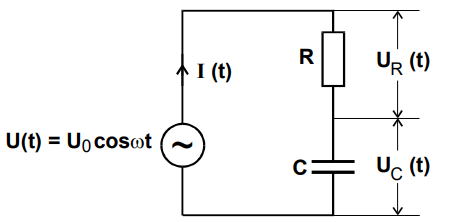
\includegraphics[height=5cm]{abbildungen/oszillatorisch.png}
    \caption{Schaltbild für den schwingenden RC-Kreis \cite{man:v353}.}
    \label{fig:schwingend}
\end{figure}

\noindent
Falls $\omega << \frac{1}{\tau}$ gilt, sind die Spannungen am Generator und am Kondensator nahezu in Phase.
Wird die Frequenz $\omega$ erhöht, so entsteht eine Phasenverschiebung $\phi$ zwischen den beiden Spannungen.
Weiterhin nimmt die Amplitude der Kondensatorspannung ab.

\noindent
Aus den Gesetzen \eqref{eq:gesetze} ergibt sich 
\begin{align}
    I(t) = \frac{\diff{Q}}{\diff{t}} = C \frac{\diff{U_\text{C}}}{\diff{t}}.
    \label{eq:stromstaerke}
\end{align}
Zusammen mit dem zweiten Kirchhoffschen Gesetz über Generator- $U$, Widerstand- $U_\text{R}$ und Kondensatorspannung $U_\text{C}$ sowie dem Ansatz 
\begin{align}
    U_\text{C} = A(\omega) \cos\left(\omega t + \phi(\omega)\right)
\end{align}
folgt schließlich 
\begin{align}
    U_0 \cos(\omega t) = -A(\omega) \cdot \omega \cdot \tau \cdot \sin\left(\omega t + \phi\right) + A(\omega) \cdot \cos\left(\omega t + \phi\right).
    \label{eq:zwischenergebnis_periodisch}
\end{align}
Dabei wird angenommen, dass die Spannungsquelle keinen Innenwiderstand hat.
Da die Gleichung \eqref{eq:zwischenergebnis_periodisch} zu jeder Zeit $t$ gelten muss,
lassen sich verschiedene Werte für $\omega t$ einsetzen.
Für $\omega t = \frac{\pi}{2}$ folgt damit für die Phasenverschiebung die Frequenzabhängigkeit
\begin{align}
    \phi(\omega) = \arctan(- \omega \tau).
    \label{eq:phasenverschiebung}
\end{align}
Für kleine $\omega$ geht $\phi$ gegen 0, für große $\omega$ asymptotisch gegen $\frac{\pi}{2}$.
Im Falle $\omega = \frac{1}{\tau}$ gilt $\phi = \frac{\pi}{4}$.

\noindent
Außerdem ergibt sich mit $\omega t + \phi = \frac{\pi}{2}$ die Spannungsamplitude
\begin{align}
    A(\omega) = - \frac{\sin(\phi)}{\omega \tau} U_0
    \label{eq:sinusgleichung}
\end{align}
am Kondensator.
Zusammen mit Gleichung \eqref{eq:phasenverschiebung} folgt hieraus schließlich
\begin{align}
    A(\omega) = \frac{U_0}{\sqrt{1+ (\omega \tau)^2}}.
    \label{eq:amplitude}
\end{align}
Die Gleichungen \eqref{eq:entladung} und \eqref{eq:amplitude} lassen sich durch eine Fouriertransformation in einander überführen.